\chapter{Elements of Computational Learning Theory}
\label{ch:computational-learning}


\section{Terminology}
\begin{itemize}
	\item \textbf{Instance space} X \(\rightarrow\) is the space from which we take the data. Is the set of instances of objects the learner wants to classify. The data from the instance space are generated through a distribution \textbf{D}, unknown to the learner.
	\item \textbf{Concepts} \(\rightarrow\) it's a collection of objects subsets of the instance space X. This should be thought of as properties of objects.
	\item \textbf{Concepts class} \(\rightarrow\) Collection of concepts
	\item \textbf{Target Concept} \(\rightarrow\) it's the concept the learner wants to build a classifier for
	\item \textbf{Representation class} \(\rightarrow\) we talk about representation class when we have a concept with non constant space to represent it, it requires size(e) bits with \(e \in C\).
\end{itemize}

\section{The General Model}
Every learning algorithm is designed to learn concepts from a concept class C but it does not know the target concept c, nor the associated distribution D.\\
The interface of every learning algorithm can be described in the following way
\begin{figure}[H]
	\centerline{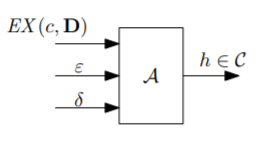
\includegraphics[scale=1]{figures/old/learning}}
\end{figure}
\begin{itemize}
	\item \(\epsilon\) is the \textbf{error parameter}, while \(\delta\) is the \textbf{confidence parameter}.
	\item EX(c,D) is called the \textit{oracle}, a procedure that A can call as many times she wants, and which return an element x from the distribution D, labelled according to whether it is in c or not. Think of it as labeled data.
	\item The error of any \(h \in C\) is defined as \(error_{D,c} = Pr_{x\sim D}[h(x) \ne c(x)]\)
\end{itemize}
So the general model will be:
\begin{figure}[H]
	\centerline{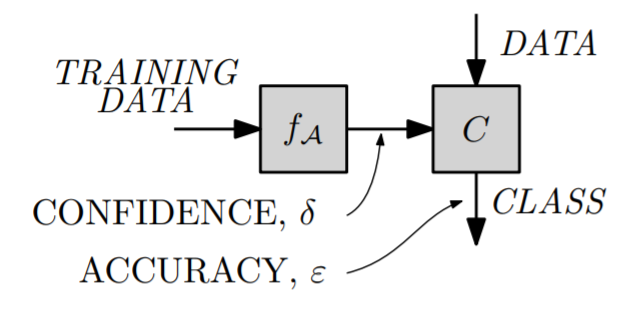
\includegraphics[scale=0.5]{figures/old/learning1}}
\end{figure}
1-\(\delta\) is the probability for which we obtain a classifier with accuracy <\(\epsilon\) .\\
\section{PAC learnable and efficiently PAC learnable}
PAC learnable is the equivalent of a function that can be computed, of a language that can be decided. A concept class is PAC learnable if there is an algorithm that can learn it. If the rime complexity of A is bounded by a polynomial in \(\frac{1}{\epsilon}\) and \(\frac{1}{\delta}\) we say that C is efficiently PAC learnable. The complexity of A is measured taking into account the number of calls to the oracle.

\section{The PAC learning model}

\begin{note}
	A Reference is given by Chapter 2 of \citet{Mohri2018}\sidecite{Mohri2018}

\end{note}

We first introduce several definitions and the notation needed to present the PAC
model.

We denote by $\mathcal{X}$ the set of all possible examples or instances.
$\mathcal{X}$ is also sometimes referred to as the \textbf{input space} or \textbf{instant space}.
The set of all possible \textbf{labels} or target values is denoted by $\mathcal{Y}$.
For the purpose of this introductory treatment, we will limit ourselves to the case where $\mathcal{y}$ is reduced to two labels, $\mathcal{Y} = \binset$, which corresponds to the so-called binary classification.
The results can then be extended to generalized version of $Y$.

A \textbf{concept} $c: \mathcal{X} \to \mathcal{Y}$ is a mapping from $\mathcal{X}$ to $\mathcal{Y}$.
Since $\mathcal{Y} = \binset$, we can identify $c$ with the subset of $\mathcal{X}$ over which it takes the value 1.
Thus, in the following, we equivalently refer to a concept to learn as a mapping from $\mathcal{X}$ to \binset, or as a
subset of $\mathcal{X}$.
As an example, a concept may be the set of points inside a triangle
or the indicator function of these points. In such cases, we will say in short that
the concept to learn is a triangle.

A \textbf{concept class} is a set of concepts we may wish to learn and is denoted by $\mathcal{C}$. This could, for example, be the set of all triangles in the plane.
We assume that examples are independently and identically distributed (i.i.d.)
according to some fixed but unknown distribution $\mathcal{D}$.

The learning problem is then formulated as follows.
The learner considers a fixed set of possible concepts
$\mathcal{H}$, called a \textbf{hypothesis set}, which might not necessarily coincide with $C$.
It receives a sample $S = (x_1,...,x_m)$ drawn i.i.d. according to $\mathcal{D}$ as well as the labels
$(c(x_1),...,c(x_m))$, which are based on a specific target concept $c \in C$ to learn. The
task is then to use the labeled sample $S$ to select a hypothesis $h \in \mathcal{H}$ that has a
small generalization error with respect to the concept $c$. The generalization error
of a hypothesis $h \in \mathcal{H}$, also referred to as the risk or true error (or simply error)
of $h$ is denoted by $R(h)$ and defined as follows.


\begin{definition}[Generalization error]
	Given a hypothesis $h \in \mathcal{H}$, a target concept $c \in \mathcal{C}$, and an underlying distribution $\mathcal{D}$, the generalization error or risk of $h$ is defined by
	\begin{equation}
		R(h) = \mathbb{P}_{x\sim\mathcal{D}}[h(x) \neq c(x)] = \mathbb{E}_{x\sim\mathcal{D}}[1_{h(x)\neq c(x)}],
	\end{equation}
	where $1_\omega$ is the indicator function of the event $\omega$.
\end{definition}

The generalization error of a hypothesis is not directly accessible to the learner
since both the distribution $\mathcal{D}$ and the target concept care unknown. However, the
learner can measure the empirical error of a hypothesis on the labeled sample $S$.

\begin{definition}[Empirical error]
	Given a hypothesis $h \in \mathcal{H}$, a target concept $c \in \mathcal{C}$, and a sample $S = (x_1,\ldots,x_m)$, the empirical error or empirical risk of $h$ is defined by
	\begin{equation}
		\hat{R}_S(h) = \frac{1}{m}\sum_{i=1}^m 1_{h(x_i)\neq c(x_i)}.
	\end{equation}
\end{definition}
Thus, the empirical error of $h \in \mathcal{H}$ is its average error over the sample $S$, while the
generalization error is its expected error based on the distribution $\mathcal{D}$.

\begin{definition}[PAC-learning]
	A concept class $\mathcal{C}$ is said to be PAC-learnable if there exists an algorithm $\mathcal{A}$ and a polynomial function $poly(\cdot,\cdot,\cdot,\cdot)$ such that for any $\epsilon > 0$ and $\delta > 0$, for all distributions $\mathcal{D}$ on $\mathcal{X}$ and for any target concept $c \in \mathcal{C}$, the following holds for any sample size $m \geq poly(1/\epsilon, 1/\delta, n, size(c))$:
	\begin{equation}
		\mathbb{P}_{S\sim\mathcal{D}^m}[R(h_S) \leq \epsilon] \geq 1-\delta.
	\end{equation}
\end{definition}